\section{Additional tables and figures}

\begin{table}[h]
\centering\footnotesize
\tab{heldout-pairwise}
\caption{CRPS skill of V2 against each baseline, paired over the forecasts
both made, with \R{c/ci-level}\% account-bootstrap intervals (held-out).
Positive: V2 is better. Computed post hoc from the stored forecasts.}
\label{tab:pairwise}
\end{table}

\begin{table}[h]
\centering\scriptsize\setlength{\tabcolsep}{3.5pt}
\tab{heldout-strata}
\caption{Held-out strata: \lC\% coverage (\%) and skill against B-SA+ at
\hB\ and \hC\ days. ``Origins'' counts V2's origins in the stratum.}
\label{tab:strata}
\end{table}

\begin{table}[h]
\centering\footnotesize
\tab{devho-v2}
\caption{V2 on the development and held-out splits.}
\label{tab:devho}
\end{table}

\begin{figure}[h]
\centering
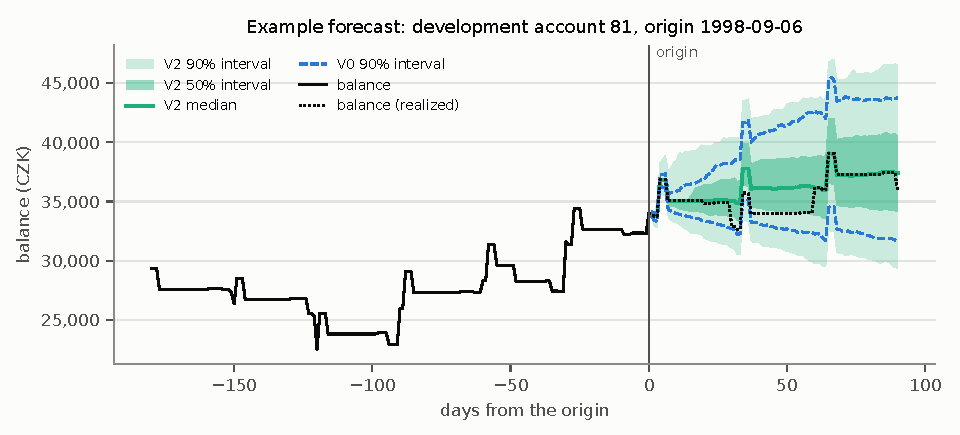
\includegraphics[width=0.85\linewidth]{figures/cone-example.pdf}
\caption{V2's and V0's \hC-day forecasts for development account
\R{fig/ex/account} at its last eligible origin (\R{fig/ex/origin}). The
account was chosen by a fixed rule (median record count among accounts with
detected income), not by look.}
\label{fig:cone}
\end{figure}

\begin{table}[h]
\centering\footnotesize
\tab{synthetic-detection}
\caption{Regime detection on synthetic data with a known change day
(\R{c/regime-seeds} seeds per scenario, detector on). Recovery: the estimate
stays within a quarter of the step for \R{c/settle-days} days. False alarms
are counted in the same seeds with no step.}
\label{tab:detection}
\end{table}

\begin{table}[h]
\centering\footnotesize
\tab{synthetic-a1}
\caption{Claim A1: V0's coverage (\%) on model-matched data with the
protocol of the engine's earlier calibration test (\R{c/a1-seeds} seeds).
The numbers reproduce that test's output exactly.}
\label{tab:a1}
\end{table}

\begin{table}[h]
\centering\footnotesize
\tab{moneydata}
\caption{MoneyData, one account, \R{md/data/eligible_origins} weekly
origins: point estimates only (one account cannot be bootstrapped by
account). V2's sparse rule never fired, so V2 equals V0.}
\label{tab:moneydata}
\end{table}

\section{Reproducing the paper}
\texttt{scripts/paper.sh} rebuilds every result from the pinned data sets,
then the figures, the numbers and this PDF. The held-out split is not
rerun: it ran once, behind its guard, and its result files are
committed. Every number in the text is read from those files by
\texttt{paper/analysis/macros.py}. The protocol, every decision and its
date, and the claims as first written are in \texttt{paper/PLAN.md}.
